\label{sec:SignalRegDef}

\subsection{Models already considered in Run-1}
Given the high increase in the center of mass energy, and therefore in the background and signal production cross sections, the signal regions used for the Run-1 analysis have to be re-optimized to maximize the sensitivity. Employing a similar methodology as in~\cite{noteSS3L}, the optimization is performed for a center-of-mass energy of $\sqrt s$~=~13~\TeV\ and a luminosity ($L$) of 3~\ifb, as a function of the $b$-jet and lepton multiplicities. The discriminating variables used to separate the signal from the background are \met, \meff, number of jets and leptons, and their \pt\ threshold. In Table~\ref{tab:SR_Paper2015} the previous defined signal regions are presented, and further used as a benchmark.


\begin{table}[htb!]
\caption{Definition of the signal regions for the Run-1 two same-sign and three leptons analysis. The cuts for the discovery and exclusion cases are shown separately. For all signal regions, two same-sign or three leptons with \pt~$>$~[20,15,15] \GeV\ are required. Jets ($b$-jets) are selected with $\pt > $ 40 \GeV\ (20 \GeV). }
\hspace{0.5cm}
\label{tab:SR_Paper2015} 
\centering
\resizebox{\textwidth}{!}{
\begin{tabular}{|c|c|c|c|c|}  
\hline
\hline
 { Signal region} 
&  $N_{lept}$ 
&  $N_{b jets}^{20}$ 
& { Signal cuts (exclusion)} 
& { Additional cuts (discovery)} \\
\hline
\hline
SR3b 
& $\ge$ 2
& $\ge $3 
& $N_{jets}^{40} \ge$ 5
& \meff $>$350~\GeV \\
\hline
 SR1b 
& ==2 
& $\ge $1 
& $N_{jets}^{40} \ge$ 3, \met\ $>$ 150~\GeV,  \mt $>$100~\GeV, !SR3b  
& \meff $>$700~\GeV \\
\hline
 SR0b 
& ==2
& ==0     
& $N_{jets}^{40} \ge$ 3, \met $>$ 150~\GeV,  \mt$>$ 100~\GeV 
& \meff $>$400~\GeV  \\
\hline
 SR3Lep low\met
& $\ge 3$
 &  -    
& $N_{jets^{40}} \ge$ 4, 50~$<$ \met $<$ 150~\GeV, Z $m_{invm}$ veto, !SR3b 
 & \meff $>$400~\GeV   \\
\hline
 SR3Lep high \met
& $\ge 3$ 
&  -    
& $N_{jets}^{40} \ge$ 4, \met $>$ 150~\GeV, !SR3b  
& \meff $>$400~\GeV\\
\hline
 \end{tabular}
}
\end{table}

The optimization is performed using as figure of merit the signal discovery significance (Zn). This is calculated with {\tt RooStats::NumberCountingUtils::BinominalObsZ}. This function requires as inputs the observed number of events (equals to SUSY signal plus SM background), the expected SM background events, and the uncertainty on these SM background expectation (40$\%$). For a complete coverage, three different approaches for the lepton selection are considered: 
\begin{itemize}
\item{Inclusive SS leptons: at least two same sign leptons are considered in the event.}
\item{Exclusive SS leptons: exactly two same sign leptons.}
\item{Exclusive three leptons: exactly three leptons.}
\end{itemize}
The cut on number of $b$-jets in the signal regions is also optimized, and four different cases are studied: 
\begin{itemize}
\item{Inclusive 3 $b$-jets: at least three $b$-jets in the event.}
\item{Exclusive 1 $b$-jet: similarly to Run-1 SR1b. It requires at least one $b$-jet, and no event with $\ge$3 $b$-jets and several jets. The latter cut is considered to mimic a potential SR3b signal region.}
\item{Inclusive 1 $b$-jet: at least one $b$-jet and no requirement on the events with three $b$-jets.}
\item{Exclusive 0 $b$-jet: no $b$-jet requirement is considered in the event.}
\end{itemize}
The final signal regions definition is chosen by looking at the signal significance, after comparing the inclusive and exclusive potential signal regions. It is a balance between a high sensitivity and a reduced number of final regions. As a result of the optimization, only four SRs are defined, and presented in Table~\ref{tab:SRdef1}. The signal region with an inclusive lepton selection and at least three $b$-jets is defined to cover the region of the SUSY phase space with a high gluino mass. For the compressed spectra, an additional signal region will be defined, as shown in the results section. Compared to the previous signal regions, the combined SR3Lep and the exactly two same sign leptons SR1b or SR0b signal regions are replaced by inclusive same sign leptons SR1b and SR0b. This retains a more simple analysis, suitable to analyze the first data. Two overlapping regions are defined for the selection with no $b$-jets in the event, and assure a high sensitivity in models with gluino mediated squarks and direct squarks. Sr0b5j is defined for SUSY signatures like gluino pair production via $WZ$, while SR0b3j for signals like direct squarks via sleptons. If no separation in terms of jet multiplicity is performed, the reached sensitivity is generally decreased by a factor 2 for the studied models. The signal region with at least one $b$-jet is orthogonal to SR0b5j and SR0b3j, and targets the signatures with 1 or 2 b jets in the cascade decays. When compared to the performance obtained with the Run-1 SRs, an increase in significance is observed (see the results section).


\begin{table}[htb!]
\caption{Preliminary signal regions definition. The two leading leptons are required to have \pt~$>$~20~\GeV.}
\hspace{0.5cm}
\label{tab:SRdef1}
\centering
\begin{tabular}{|c|c|c|c|}
\hline
\hline
Signal region  &      $N_{lept}$             & $N_{b-jets}^{20}$               & Other variables \\
\hline
\hline
SR3b     &   $\ge$2  &   $\ge$3        &    $N_{jets}^{40} \ge$ 6       \\
\hline
SR1b     &  $\ge$2  &    $\ge$1        &     $N_{jets}^{50} \ge$ 4, \met\ ~$>$~150 \GeV, \meff\ $>$ 500 \GeV \\
\hline
SR0b5j &  $\ge$2  &    $==$0        &     $N_{jets}^{50} \ge$ 5, \met\ ~$>$~100 \GeV, \meff\ $>$ 400 \GeV \\
\hline
SR0b3j &  $\ge$2  &    $==$0        &     $N_{jets}^{40} \ge$ 3, \met\ ~$>$~200 \GeV, \meff\ $>$ 400 \GeV \\
\hline
\end{tabular}
\end{table}

\begin{table}[htb!]
\caption{Inclusive lepton and $b$-jets SR1b signal region definition.}
\label{tab:def_SR1b_inclLepB}
\centering
\begin{tabular}{|c|c|c|c|}
\hline
\hline
  Signal region      &   $N_{lept}$  & $N_{b-jets}^{20}$   & Other variables \\
\hline
SR1b(inclusive)  &   $\ge$ 2       &  $\ge$ 1        &  $N_{jets}^{40}$ $\ge$ 4, \met\ $>$ 150 \GeV, \meff\ $>$ 900 \GeV    \\
\hline
\end{tabular}
\end{table}


\begin{figure}[htb!]
\centering
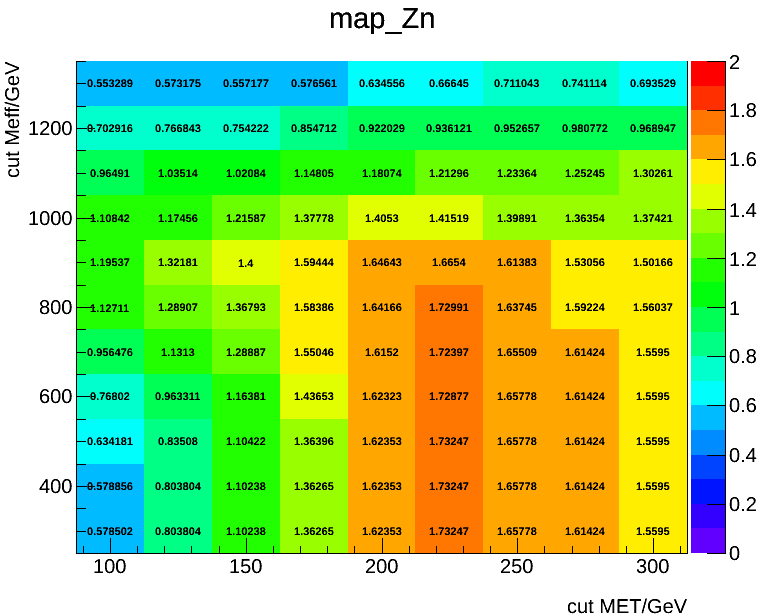
\includegraphics[width=0.6\textwidth]{FIGURES/map_MET_Meff_Gtt.png}
\caption{The \met\ and \meff\ cuts optimization. The signal significance (Zn) is calculated for the signal point with a gluino mass of 1300 GeV and LSP mass of 700 \GeV\ (gluino mediated virtual stop model). The event selection requires at least two leptons with \pt\ of [20, 20, 10] \GeV, at least 4 jets with \pt~$>$~40 \GeV\ and at least one $b$-jet with \pt~$>$~20 \GeV. For this point the reached significance with SR1b(inclusive) is 1.4, with a expected signal yield of 5.2 events. %The expected fake lepton background is 2.89, while the prompt SS background of 3.38 when considering $L$~=~3~\ifb.
}
\label{fig:map_MET_Meff_Gtt}
\end{figure}

\begin{figure}[htb!]
\centering
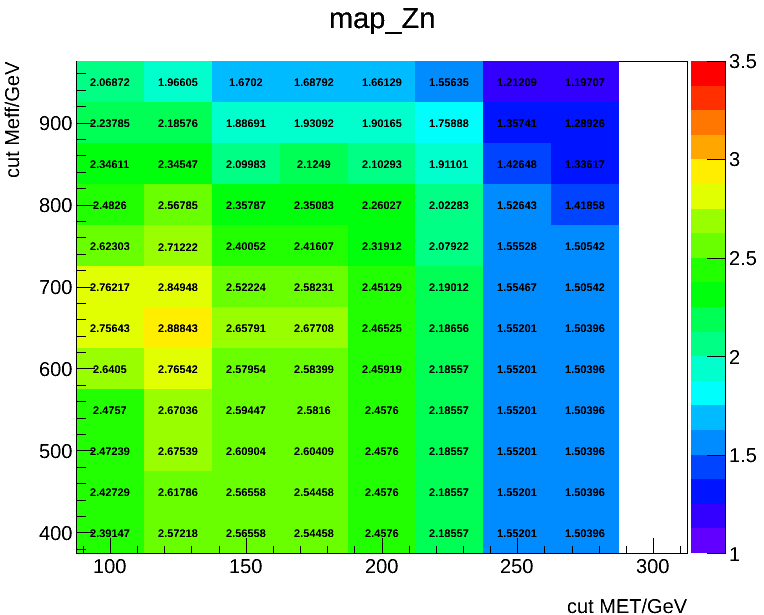
\includegraphics[width=0.6\textwidth]{FIGURES/map_MET_Meff_Sbottom.png}
\caption{The \met\ and \meff\ cuts optimization. The signal significance (Zn) is calculated for the signal point with a sbottom mass of 550 GeV and $\chi_1^{\pm}$ ($\chi_1^0$) mass of 150 (60) \GeV\ (direct sbottom model). The event selection requires at least two leptons with \pt\ of [20, 20, 10] \GeV, at least 4 jets with \pt~$>$~40 \GeV\ and at least one $b$-jet with \pt~$>$~20 \GeV. For this point the reached significance with SR1b(inclusive) is 1.88, with an expected signal yield of 9.2 events. }
\hspace{0.5cm}
\label{fig:map_MET_Meff_directSb}
\end{figure}

\paragraph{Inclusive same  sign leptons and 1 $b$-jet signal region\\}
During the optimization, a combined version of {Run-1 SR1b and SR3b} signal regions was also considered (the inclusive 1 $b$-jet case presented previously). This study is performed looking at gluino mediated virtual stop and direct sbottom models with RPC and $\chi_1^0$ being the LSP, as generally motivated by \textit{natural SUSY}. The optimization results are pointing to the generally favoured selection presented in Table~\ref{tab:def_SR1b_inclLepB}. It requires at least 4 jets, $\met>150$~\GeV and a tight cut on \meff\ to reduce the background and increase the sensitivity at high gluino and low LSP masses. 
The expected fake lepton background is 2.89, while the prompt SS background of 3.38 when considering $L$~=~3~\ifb. 
This region is not suitable in the compressed region of (see Figure~\ref{fig:map_MET_Meff_Gtt}, where only a significance of 1.4 can be achieved for a mass splitting of 600~GeV between gluino and neutralino), or in the non-excluded region of the direct sbottom model (Figure~\ref{fig:map_MET_Meff_directSb}, which is showing one the signal points with larger significance for this model, and it can only reach values of 1.88). 
The optimization is still work in progress, and the signal region definition might change. 
Work is ongoing to define a signal region targeting theses regions of the phase space. 
%A signal region targeting these regions of the phase space is work in progress. 

\subsection{Softer selection with 3$b$-jets} 

It was noticed in the 8~\TeV signal samples for the gluino stop offshell model with the most compressed mass spectrums, 
that the signal acceptance could be significantly increased for a similar level of background, by relying on softer jets (20~\GeV instead of 40~\GeV), 
but increasing the requirements on the multiplicity ($\geq 7$ jets was found optimal). 
We are considering the possibility of implementing such a signal region, which could for example take the form of the jet multiplicity distribution 
in events with two same-sign leptons and three $b$-jets. 
The expected number of events for such a distribution can be found in section~\ref{sec:fit}, 
together with estimates of the sensitivity this signal region would bring. 

\subsection{3L3b} 
%\FloatBarrier
%\clearpage
\label{sec:3l3b}

\par Given the features observed in events with  three leptons and
three b-tagged jets (3L3b) int the 20.3~$fb^{-1}$ of 8 TeV
data~\cite{3l3b}, we would like to revisit this region in Run-2 using
13~\TeV\ data. The signal regions on the 2012 search do not cover the
kinematic phase space of the 3L3b sample. Therefore, we would like to
introduce a signal region so that the entire phase space of the 3L3b
sample is considered as a signal region.  

\par We would also like to evaluate the sensitivity of our signal
regions to processes that might give rise to the excess observed in
the 3L3b sample. A popular simplified compressed SUSY model that might
give rise to such signal candidates is 
gluino-stop offshell $\gluino\to t\bar t\neut$ model described in 
Section~\ref{sec:signal} 
%he pair production of gluinos
%which further decay with a 100\% decay branching ratio via stops
%(\stop) into a final state of four top quarks and two neutralinos
%(\neut) 
(Fig.~\ref{fig:feynman_3rdgen}). 
It is assumed that the
squarks of the first two generations are much heavier than the gluino
and thus decoupled. This decay can be targeted by multiple signatures
as seen in Figure Fig~\ref{fig:run1excl_3rdgen}. One particular
process of interest is the $n$-body decay of $\gluino\to t\bar{t}\neut$
mediated by an off-shell top squark where the final state produces
four $W$-bosons and four $b$ quarks. This process has at least two
free parameters, the gluino and neutralino masses, and thus it is
important to cover all the accessible phase space with the first
13~\TeV\ data. For now, we used signal simulations 8~\TeV\ collisions
with $m_{\gluino}-m_{\neut} \geq 2 m_t$. A region of interest that was
investigated by ATLAS recently~\cite{Maurer:1966089} but was not covered in the search is
$(m_t+m_W+m_b) < (m_{\gluino}-m_{\neut})< 2m_t$ as shown in
Fig.~\ref{fig:run1excl_3rdgen}. However, it was studied by
CMS~\cite{cms_summ}.
The gluino decays to a neutralino with one off-shell top which looks
at more compressed spectra, the so-called "above the diagonal"
region. This region is especially interesting for the same-sign or
three leptons analysis since the sensitivity of this channel is better
than the other channels based on extrapolating the limits of
Fig.~\ref{fig:run1excl_3rdgen}.
 
\par The first case in the gluino decay mode is a 3-body decay with two
on-shell top quarks $\gluino\to t\bar t\neut$. This region was covered
by the ATLAS search. When the mass difference between the gluino and
neutralino goes below $2m_t$, not all the top quarks that are
produced from the gluino decay stay on-shell. The next possible decay
modes are the 4-body decay $\gluino\to\bar{b}W^-t \neut$ and the
5-body decay $\gluino\to\bar{b}W^-bW^+ \neut$. The more final
particles there are, the smaller the decay width and thus the longer
the gluino lifetime. Fig.~\ref{fig:virtual} illustrates these
processes where the ratio of the gluino decay width for each n-body
decay to the most inclusive mode, 7-body decay, is shown as a function
of the neutralino mass.

\begin{figure}[htb]
\centering
\subfigure{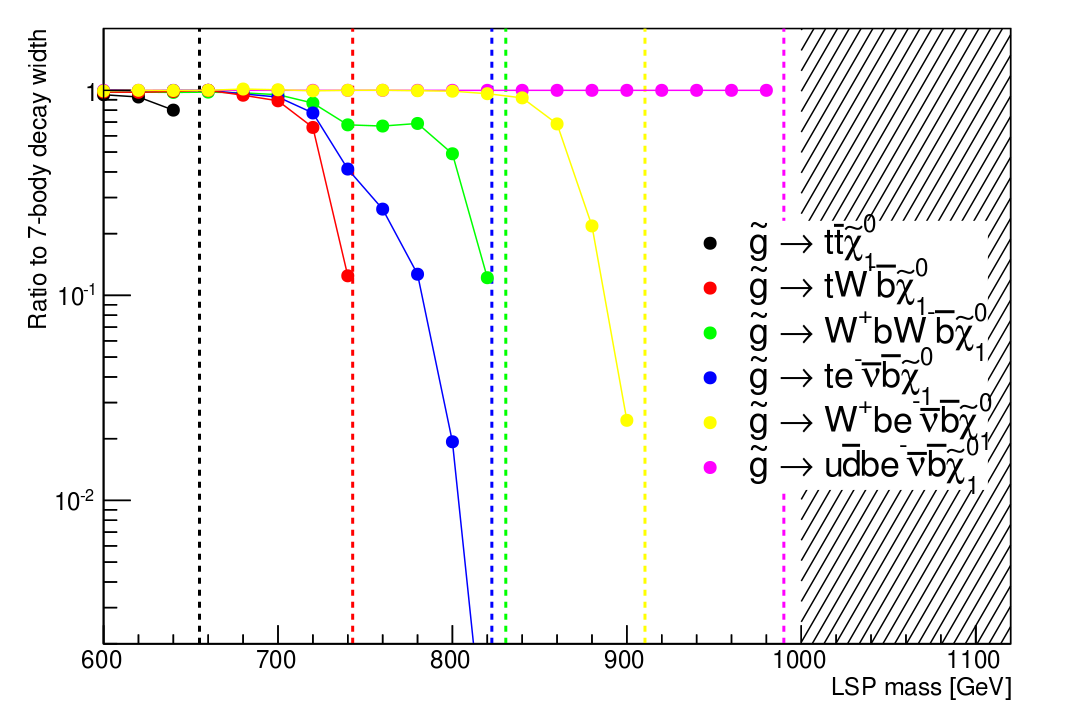
\includegraphics[width=0.47\textwidth]{fig_3L3b/virt_n_body}}
\subfigure{\includegraphics[width=0.49\textwidth]{fig_3L3b/gl_lifetime}}
\caption{(Left) Virtuality of the top quarks and $W$ bosons in the
gluino decay presented as the ratios of decay width between modes
forcing on-shell top quarks or $W$ bosons, and the most inclusive mode
(7-body decay) with no such constraints as a function of the
neutralino mass with the gluino mass fixed at 1 TeV, and stops $\tilde{t}_{1}$, $\tilde{t}_{2}$
masses are both set to 2.5~TeV with a mixing angle of
45$^\circ$. (Right) gluino lifetime as a function of the neutralino
mass for different gluino mass points.}
\label{fig:virtual}
\end{figure}

\par The gluino might live long enough to decay
to leptons that do not originate from the primary vertex,
$d_0>100$~$\mu$m, as illustrated in Fig.~\ref{fig:virtual}. Typically,
the gluino should live less than about a picosecond in order to decay
with prompt leptons. Fig.~\ref{fig:gl_lifetime} shows the gluino
lifetime as a function of the neutralino mass for different gluino
masses that will be considered in this study.

\begin{figure}[h!]
\centering
\subfigure{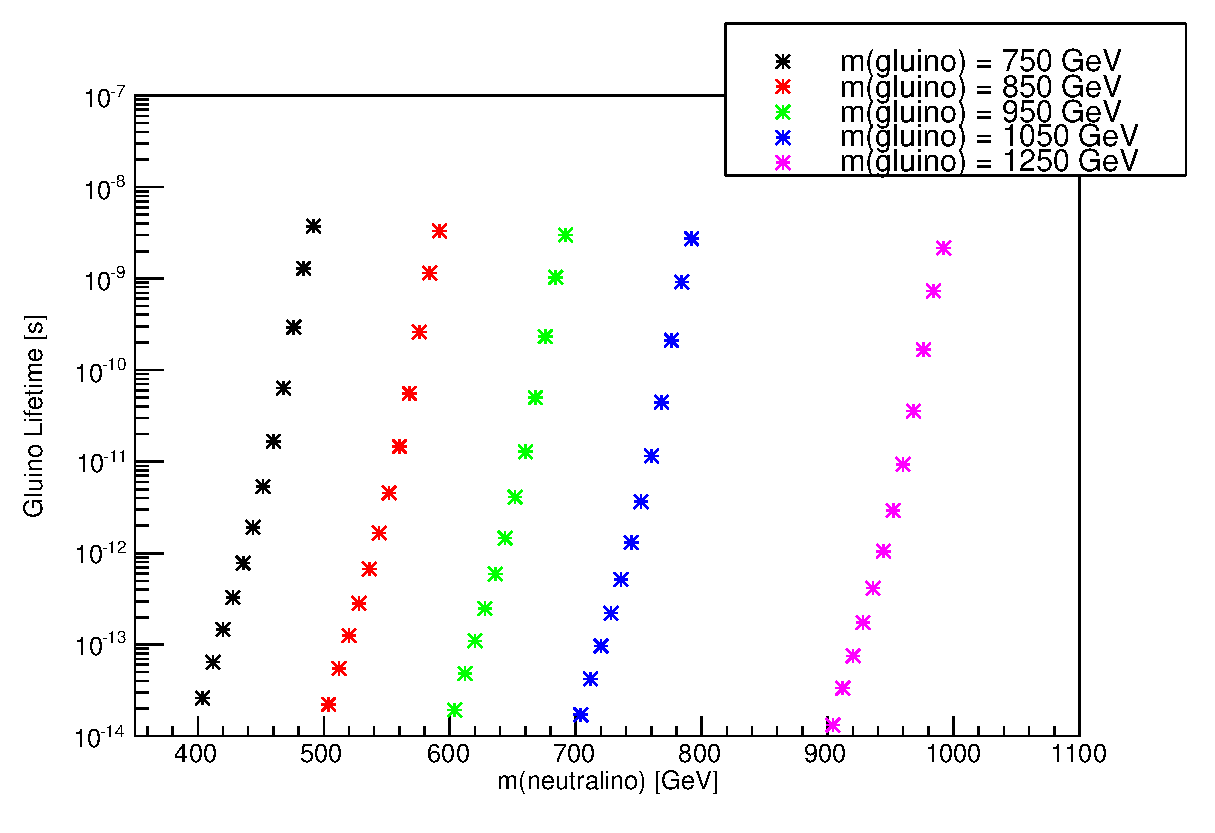
\includegraphics[width=0.65\textwidth]{fig_3L3b/grid_mass.eps}}
\caption{ Lifetimes of gluinos with different masses as a function of the neutralino mass considered in the current study. The lightest stop mass is fixed to 2.5 TeV and is a $t_L$ state.}
\label{fig:gl_lifetime}
\end{figure}

As shown in Fig.~\ref{fig:virtual} and Fig.~\ref{fig:gl_lifetime}, it
is clear that the smaller the mass gap between the gluino and
neutralino, the longer the lifetime. More details about the dominant
gluino decay modes and lifetimes can be found
in \cite{Maurer:1966089}. To evaluate the sensitivity of our signal
regions to this specific process, we used reconstructed simulations of
different mass points to evaluate how many events will pass the
standard SS/3L analysis event selection. The grid points were chosen
so that for a fixed gluino mass, two neutralino masses were taken to
be closer and farther from the diagonal in the region with
$m_{\gluino}-m_{\neut} < 2 m_t$ as shown in
Table~\ref{tbl:gl_selected_lifetime}.


\begin{table*}[htb]
\begin{center}
\setlength{\tabcolsep}{0.0pc}
\caption{Gluino decay width  $\left[\GeV\right] $ and lifetime (s) for \mass{\stop} = 2500 \GeV   and for different pairs of $( \mass{\gluino} \left[\GeV\right], \xspace \mass{\neut} \left[\GeV\right])$.}
\label{tbl:gl_selected_lifetime}
{\footnotesize
%%
{
%\centering
\begin{tabular*}{\textwidth}{@{\extracolsep{\fill}}lcccccc}
  \noalign{\smallskip}\hline\noalign{\smallskip}\hline
  &  $\left( 750, \spl{435}{485} \right)$ & $\left( 850,   \spl{535}{585} \right)$  & $\left( 950,   \spl{635}{685} \right)$ & $\left( 1050,   \spl{735}{785} \right)$ &  $\left( 1250,   985 \right)$\\ 
\noalign{\smallskip}\hline\noalign{\smallskip} \hline
%%
  Gluino Decay Width $\left[\eV\right] $    & \spl{9.4$\times10^{-4}$}{4.4$\times10^{-7}$}         & \spl{1.1$\times10^{-3}$}{5.1$\times10^{-7}$}        &    \spl{1.2$\times10^{-3}$}{5.6$\times10^{-7}$}       &  \spl{1.4$\times10^{-3}$}{6.1$\times10^{-7}$}          &    7.7$\times10^{-7}$    \\
\noalign{\smallskip}\hline\noalign{\smallskip}
     Gluino Lifetime (picoseconds)     & \spl{0.7}{1500}          & \spl{0.6}{1300}        &    \spl{0.5}{1200}       &  \spl{0.5}{1100}          &    860     \\
 \noalign{\smallskip}\hline\noalign{\smallskip}\hline
%%
\end{tabular*}
}
}
%%%
\end{center}
\end{table*}

The event selection of 3L3b follows:

\begin{itemize}
\item exactly 3 baseline leptons are required with at least one pair of opposite sign same flavour (OSSF)
\item the missing transverse momentum is required to be greater than 50 \GeV
%\item events with an OSSF that satisfies $81.2 \GeV < m_{ll} < 101.2 \GeV$  or $81.2 \GeV < m_{lll} < 101.2 \GeV$ are discarded
\item the events are required to have at least three b-jets.
\end{itemize}

In order to cover the kinematic region of the 3L3b selection, a new signal region is added in the SS/3L analysis that is still orthogonal to rest of the signal regions. This new signal region requires exactly three leptons, at least three b-jets and either at most five jets or $M_{eff} < 350 \GeV$ and we refer to it as SR3b3L.  
The final signal regions used in this study are shown in Fig.~\ref{tab:SR_Paper2015}.

Appendix~\ref{app_above_diag} shows the generated samples used in this study. The event yields for the grid points considered that pass the selection requirements in the different signal regions and normalized to the 13 \TeV cross section with 3~$fb^{-1}$ are shown in Table~\ref{tbl:yields_sr}.


\begin{table*}[htb]
\begin{center}
\setlength{\tabcolsep}{0.0pc}
\caption{ Number of events passing the selections for \mass{\stop} = 2500 \GeV and for different pairs of $(\mass{gl} \left[\GeV\right], \xspace \mass{\neutralino} \left[\GeV\right] )$ normalized to 
13 \TeV with  3~$fb^{-1}$.
}
\label{tbl:yields_sr}
{\footnotesize
%%
{
%\centering
\begin{tabular*}{\textwidth}{@{\extracolsep{\fill}}lcccccc}
  \noalign{\smallskip}\hline\noalign{\smallskip}\hline
{\bf Signal Regions}  &  $\left( 750, \spl{435}{485} \right)$ & $\left( 850,   \spl{535}{585} \right)$  & $\left( 950,   \spl{635}{685} \right)$ & $\left( 1050,   \spl{735}{785} \right)$ &  $\left( 1250,   985 \right)$\\ 
\noalign{\smallskip}\hline\noalign{\smallskip} \hline
%%
 SR3b3L  & \spl{6.71}{3.48}&    \spl{3.44}{1.46}        &    \spl{2.03}{0.57}       &  \spl{0.78}{0.29}          &    0.07    \\
\noalign{\smallskip}\hline\noalign{\smallskip}
SR3b         & \spl{6.03}{1.44}          & \spl{2.35}{0.45}        &    \spl{0.80}{0.14}         &  \spl{0.46}{0.05}          &     0.02    \\
\noalign{\smallskip}\hline\noalign{\smallskip}
SR1b         & \spl{1.02}{1.61}          & \spl{0.67}{1.16}       &    \spl{0.42}{0.47}        &  \spl{0.21}{0.22}          &     0.04  \\
\noalign{\smallskip}\hline\noalign{\smallskip}
SR0b         & \spl{7.81}{5.44}          & \spl{4.30}{1.94}        &    \spl{1.50}{1.01}        &  \spl{0.81}{0.41}          &    0.12    \\
\noalign{\smallskip}\hline\noalign{\smallskip}
SR3Llow         & \spl{1.20}{3.07}          & \spl{0.97}{0.41}     &    \spl{0.43}{0.11}         &  \spl{0.24}{0.07}          &    0.01   \\
\noalign{\smallskip}\hline\noalign{\smallskip}
SR3Lhigh         & \spl{1.95}{2.46}          & \spl{1.46}{0.67}    &    \spl{0.52}{0.40}        &  \spl{0.28}{0.24}          &    0.04     \\
 \noalign{\smallskip}\hline\noalign{\smallskip}\hline
%%
\end{tabular*}
}
%%%
}
\end{center}
\end{table*}
%

%{\bf sasha, should we add the yields normalized to cross section? in this case for 8 tev we are not sensitive, but we could scale the cross section for 13 tev and show these numbers since they are more relevant? Perhaps we can find a working point for integrated luminosity where we will become sensitive.}

The kinematic distributions of $N_{jets}$, $N_{b-jets}$, $\met$, and $M_{eff}$ are shown in Fig.~\ref{fig:3l3b_distributions}. The $N_{jets}$ distribution peaks at 2 jets, thus it useful to use the new signal region, SR3b3L, which cover the lower jet multiplicity. The $\met$ peaks at around 60~\GeV and thus motivates the lower cut of 50~\GeV in this same signal region. The current cuts in $M_{eff}$ of 350~\GeV cover the signal well. 


\begin{figure}[htb!]
\centering
\subfigure{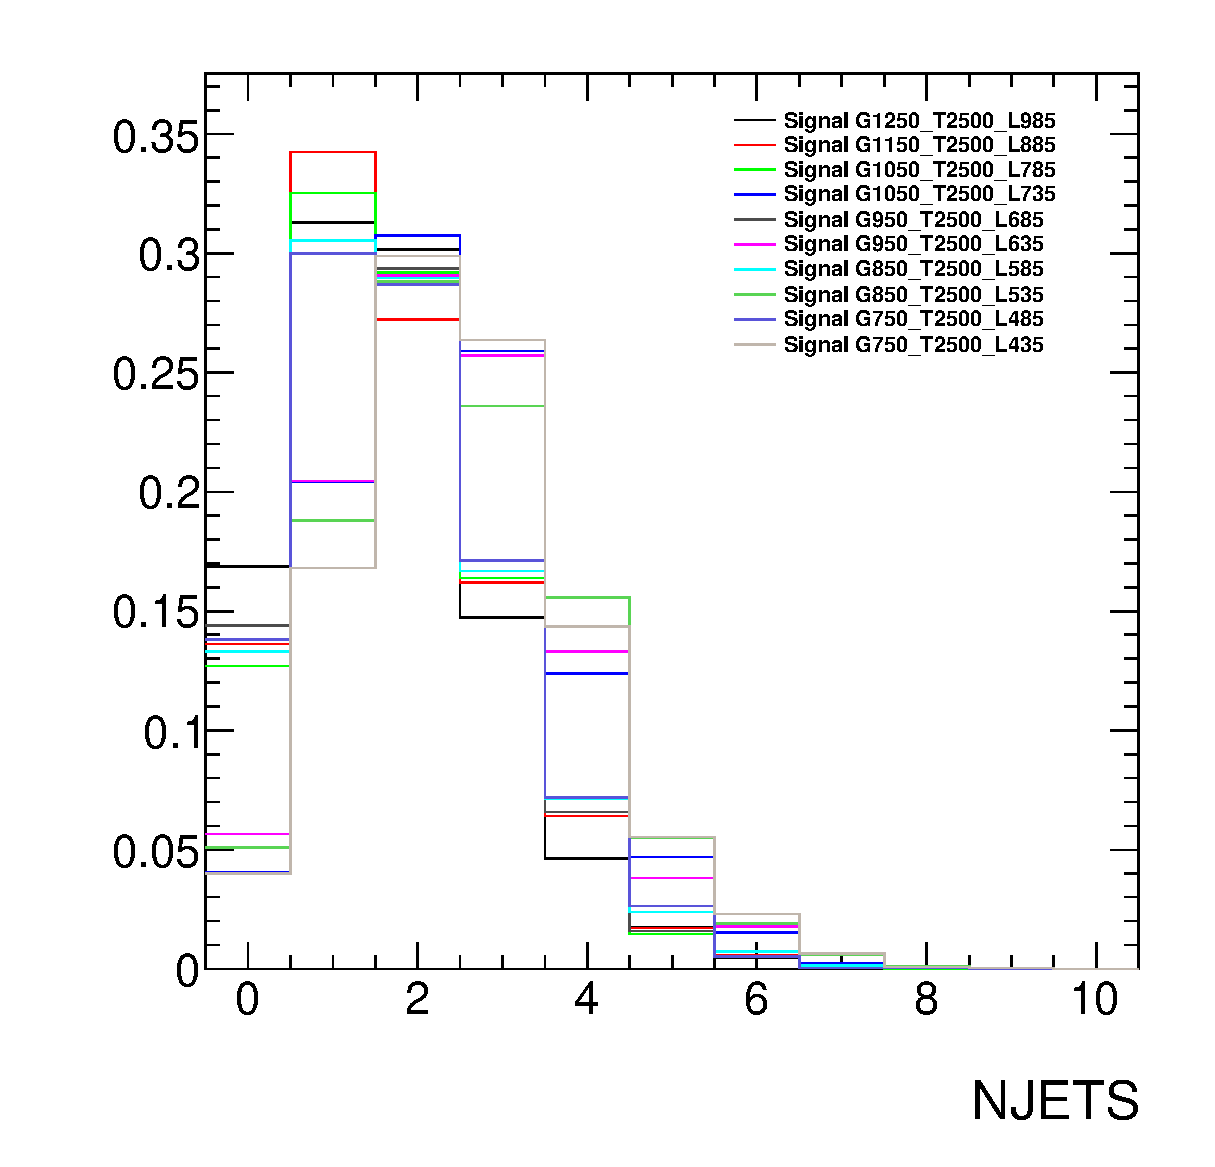
\includegraphics[width=0.4\textwidth]{fig_3L3b/num_jets.eps}}
\subfigure{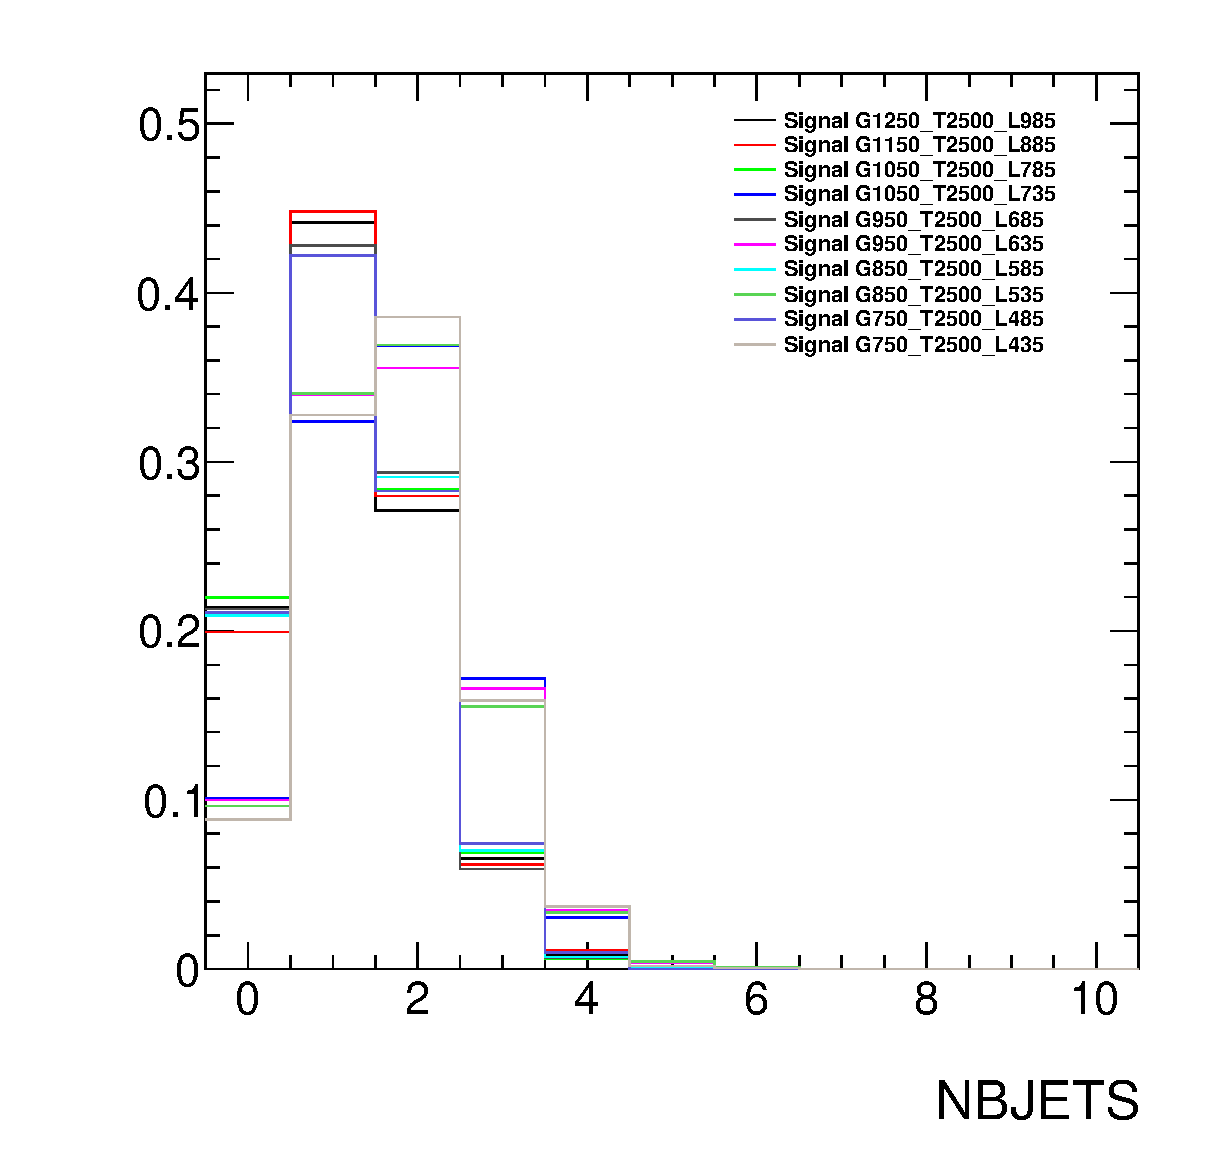
\includegraphics[width=0.4\textwidth]{fig_3L3b/num_bjets.eps}}\\
\subfigure{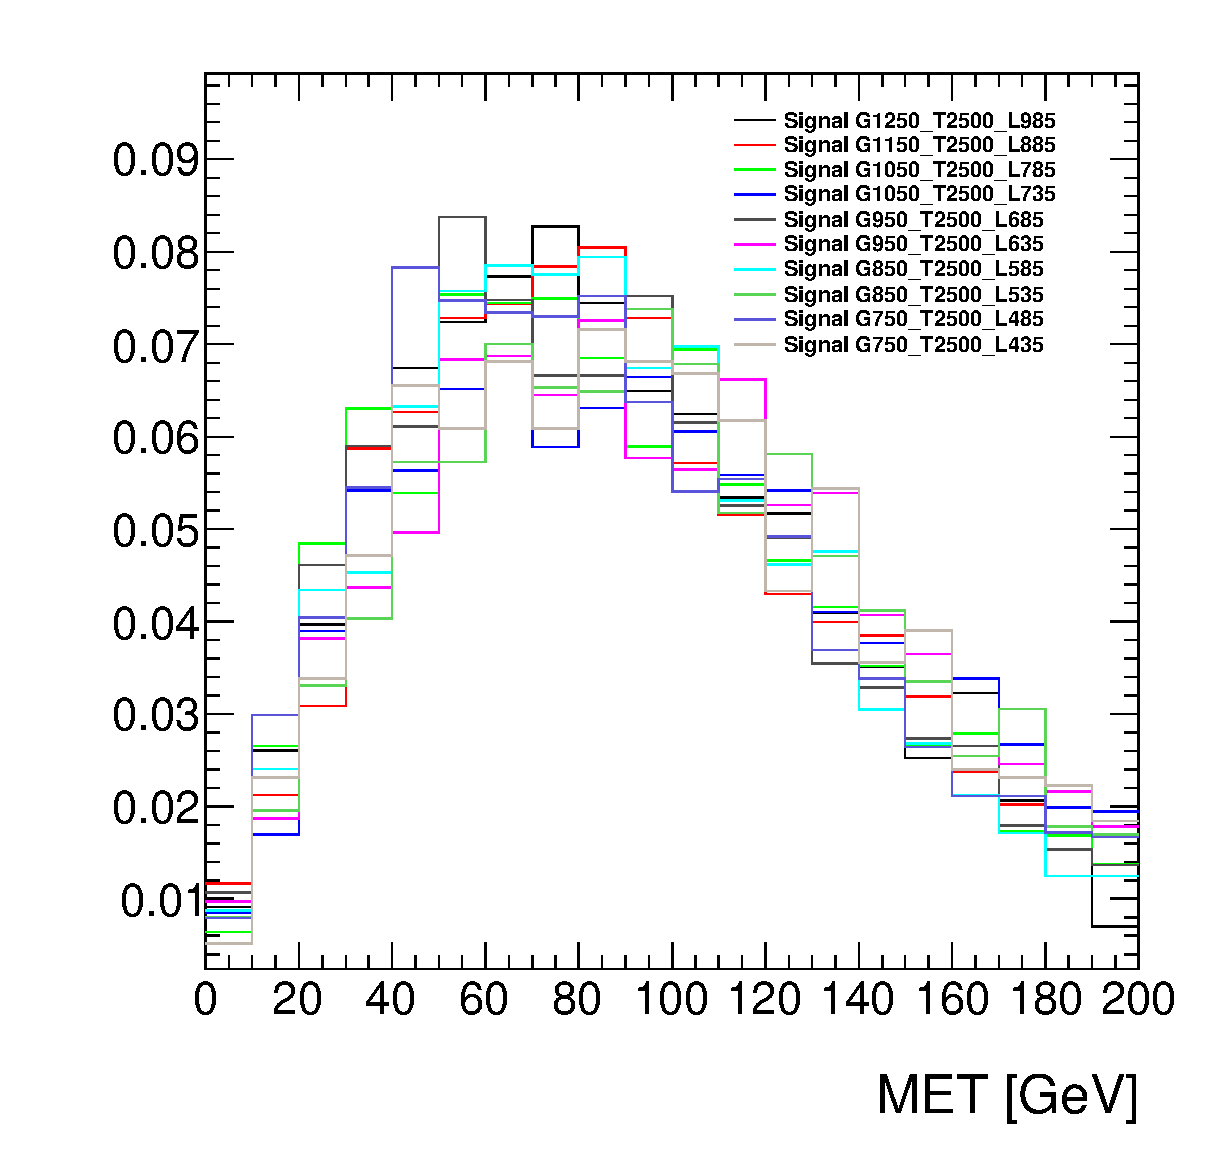
\includegraphics[width=0.4\textwidth]{fig_3L3b/met.eps}}
\subfigure{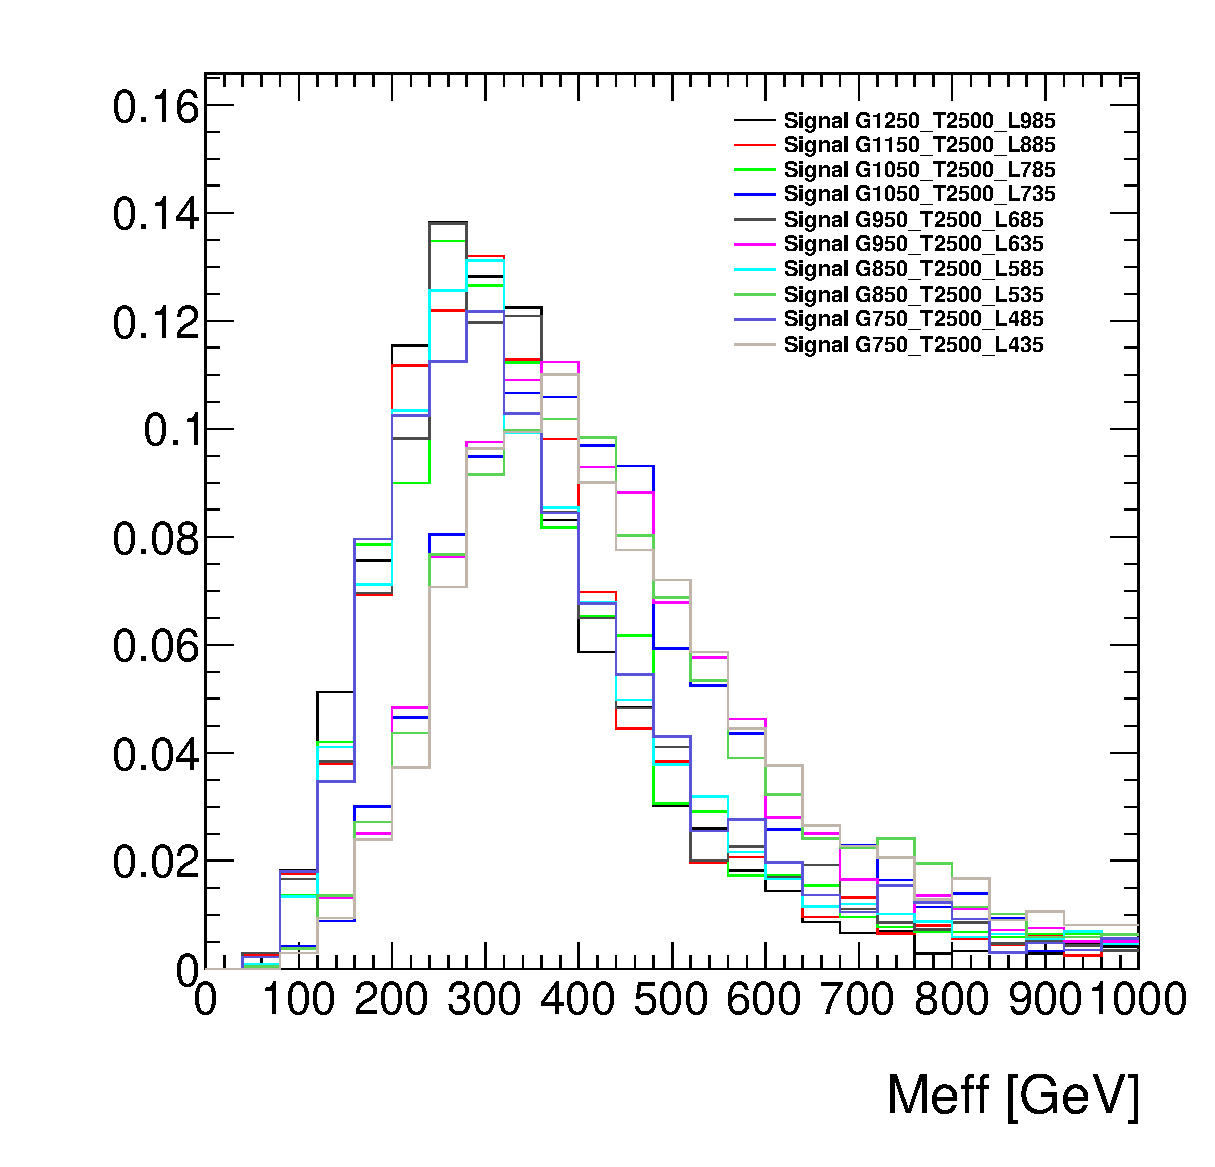
\includegraphics[width=0.4\textwidth]{fig_3L3b/meff.eps}}
\caption{ Kinematic distributions for the SS/3L channel with reconstructed samples generated at 8 \TeV}
\label{fig:3l3b_distributions}
\end{figure}



Our next step is to evaluate the background in these signal regions and determine our sensitivity with 13~\TeV data. 

%\FloatBarrier
 

\clearpage
\subsection{RPV models} 

The main topologies described in Section~\ref{subsec:RPVmodel} and shown in Fig.~\ref{fig:rpv_diagram} lead to the same final state: 
 \begin{align}
\ell^{\pm} \ell^{\pm} + b{\rm{-jets}} + {\rm{jets}} + \met
 \end{align}
 with two leptons and two $b$-jets coming from the top quarks decay, extra jets and eventually $b$-jets coming from the decay of the $d$-squark or the gluino and the \met\ coming from the neutrinos from the top quarks decay.

 An optimization of signal region for this model was performed and will be soon written out on this note. The main aspects of the optimized signal region are:
\begin{itemize}
\item $\geq 2$ leptons 
\item $\geq 1$ $b$-jets 
\item $\geq 3$ jets 
\item $H_{\rm T} = \Sigma \pt^{jet} \geq \ \sim 150$~\GeV\
\item No cut on \met\ and $M_{\rm T}$ 
\end{itemize}

 The cuts on the number of $b$-jets and jets are relaxed in order to take into account the boosted region.
 Indeed, the on-shell gluinos and $d$-squarks can be so boosted that their decay products are very close and 
 not all the jets and $b$-jets are reconstructed.

A tight cut on the overall jet activity in the event is the main cut to
reject the background. The $H_{\rm T}$ variable was chosen among other
variables, such as $H_{\rm T}' = \Sigma \pt^{jet} + \Sigma \pt^{lep}$
and $M_{\rm{eff}} = \Sigma\pt^{jet} + \Sigma\pt^{lep} + \met$, because
it leads to the best results in terms of significance.
  The exact cut value will be optimized with a future more accurate study.
  
 However, a minimal cut should be applied on \met\ and $M_{\rm T}$. These cuts were originally applied for the search for neutralinos for RPC models and to reject the main background coming from the neutrinos from the decay of $W$.
 Since in RPV models our signal is composed of neutrinos, it is necessary that these cuts should be as low as possible in order to avoid the losses in signal acceptance. 
Table~\ref{tab:RPV_SR_Significance} shows the signal acceptance Zn computed assuming a 40\% background uncertainty and 
using the signal samples at truth level. 
For those numbers, no $b$-tagging is used, and the $b$-jets were assigned according to their truth flavor in both background and signal samples.
%One can be convinced by the performance of this signal region with the Table~\ref{tab:RPV_SR_Significance}. 

\begin{table}[h!]
\caption{Yields and Significance for each additional cuts at $\sqrt{s} = 13$~\TeV for 3~fb$^{-1}$ of luminosity. The signal samples used here are a $d$-quark fusion (top) and a gluon fusion (bottom) for $\lambda''_{321}$ coupling for the respective mass points ($m_{\gluino}=2000$~\GeV,$~m_{\tilde{q}}=1400$~\GeV) and ($m_{\gluino}=800$~\GeV,$~m_{\tilde{q}}=2000$~\GeV).}
\hspace{0.5cm}
\label{tab:RPV_SR_Significance}
\centering
\resizebox{\textwidth}{!}{
\begin{tabular}{|l|c|c|c|c|c|}

\hline
	Cuts & RPV $d$-quark fusion & $Z~+~\rm{jets}$ & $t\bar{t}$ & $t\bar{t}~+~V$ & Significance\\
\hline
$N_{\ell} \geq$~2 & 70.02 $\pm$ 1.05 & 66830 $\pm$ 2557 & 14467 $\pm$ 44 & 91.83 $\pm$ 0.85 & -0.26 \\
$+$ $N_{jet} \geq$~3, $N_{b-jet} \geq$~1  & 51.96 $\pm$ 0.90 & 1697 $\pm$ 43 & 11277 $\pm$ 39 & 84.04 $\pm$ 0.81 & -0.25 \\
$+$ $H_{\rm T} >$~150 \GeV & 37.36 $\pm$ 0.76 & 1.06 $\pm$ 0.85 & 8.29 $\pm$ 1.06 & 0.53 $\pm$ 0.05 & 4.23 \\
\hline 
\hline
Cuts & RPV gluon fusion & $Z~+~\rm{jets}$ & $t\bar{t}$ & $t\bar{t}~+~V$ & Significance\\
\hline
$N_{\ell} \geq$~2 & 56.73 $\pm$ 0.90 & 66830 $\pm$ 2557 & 14467 $\pm$ 44 & 91.83 $\pm$ 0.85 & -0.26 \\
$+$ $N_{jet} \geq$~3, $N_{b-jet} \geq$~1 & 45.30 $\pm$ 0.81 & 1697 $\pm$ 43 & 11277 $\pm$ 39 & 84.04 $\pm$ 0.81 & -0.26 \\
$+$ $H_{\rm T} >$~150 \GeV & 14.89 $\pm$ 0.46 & 1.06 $\pm$ 0.85 & 8.29 $\pm$ 1.06 & 0.53 $\pm$ 0.05 & 2.00 \\
\hline

\end{tabular}
}
\end{table}
 
  
 
